\chapter{Background} \label{chap:background}
This chapter is focused on making the reader familiar with concepts used throughout this report.
First, an introduction to computational complexity is given to establish a mathematical framework to describe the efficiency of computer algorithms.
Second, the basic ideas of quantum mechanics are presented.
Finally, an overview of quantum computation is given.

\section{Computational Complexity}
In computer science, there seems to be a fundamental limit to what problems we can solve.
Some problems seem to be inherently uncomputable: there exists no general solution that does not go into an infinite loop for certain inputs~\cite{church1936note, turing1937computable}.
This report will not go further into what problems are computable and uncomputable.
Rather, it will look at the computational efficiency of certain algorithms: how many resources are required to solve a problem?

\subsection{Big-O Notation}
The time and space required by an algorithm generally grows as the size of the input grows.
Because of this, it is traditional to describe the efficiency of an algorithm as a function of the size of its input~\cite{cormen2009introduction}.
This function describes the number of primitive operations it performs for a given input size.
The notion of input size here depends on the context of the problem.
For example, when computing the discrete Fourier transform, the input size refers to the dimension of the input vector.
When talking about a problem like integer multiplication, however, it is more fitting to talk about the input size as the number of bits needed to represent the input in binary.

When analyzing the efficiency of algorithms, we look at the asymptotic growth for a given input size.
Consider an algorithm that given input size $n$ takes $n^2$ primitive operations to run and another algorithm that takes $500n^2 + \log n$ primitive operations to run.
In big-O notation, both these algorithms are said to run in $O(n^2)$ time.
That is, the number of primitive operations it performs scales quadratically with the input size.
Constant factors are ignored as they become negligible as $n \to \infty$.
While they are practically significant --- an algorithm that runs in $O(n/2)$ runs twice as fast as an algorithm that runs in $O(n)$ --- they are not relevant to asymptotic analysis. 

Formally, if we have functions $f(n)$ and $g(n)$ such that $f$ eventually grows slower than some multiple of $g$ as $n \to \infty$, we say $f(n) = O(g(n))$.
For example, given $f(n) = 200n^2$ and $g(n) = n^3$, $f$ begins to grow slower than $g$ when $n > 200$.
Thus, $g$ bounds $f$ from above, and $f(n) = O(g(n)) = O(n^3)$.
Some common big-O run times are shown in \Cref{table:common-big-o}, along with their written name and an example.
Throughout this report, algorithms that are bounded above by a polynomial (i.e. all run times until polynomial in \Cref{table:common-big-o}) will be referred to as polynomial-time algorithms, and algorithms that are not bounded above by a polynomial will be referred to as superpolynomial-time algorithms.

\begin{table}[ht]
    \centering
    {\renewcommand{\arraystretch}{1.1}
        \begin{tabular}{ c|c|c }
            Notation & Name & Example \\
            \hline
            $O(1)$ & Constant & Accessing single element from array \\
            $O(\log n)$ & Logarithmic & Binary search \\
            $O(n)$ & Linear & Unstructured database search \\
            $O(n \log n)$ & Linearithmic & Fast Fourier Transform \\
            $O(n^2)$ & Quadratic & Insertion sort \\
            $O(n^k)$ & Polynomial & Gaussian elimination \\
            $O(k^n)$ & Exponential & Graph coloring \\
            $O(n!)$ & Factorial & Brute-force search traveling salesman problem \\
        \end{tabular}
    }
    \caption{Common big-O run times from fast to slow.}
    \label{table:common-big-o}
\end{table}

\subsection{Turing Machines}
The previous section described the measurement of computational efficiency as the number of primitive operations it performs for a given input size.
This abstract definition can be extended by choosing a computational model in order to define what a primitive operation means.
The standard computational model used for this is the Turing machine.
It is chosen as computational model for the analysis of computational efficiency because of its simplicity and because it is able to simulate most physically realizable computational models with little overhead~\cite{arora2009computational}.

A Turing machine is an abstract machine that manipulates symbols from a work alphabet on a finite amount of one-way infinite length tapes divided into cells~\cite{turing1937computable}~(\Cref{fig:single-tape-turing-machine}).
Along these tapes runs a tape head that can read and write one symbol at a time.
The machine has a finite set of states, which the machine executes one at a time by loading them into the state register.
At any time, the machine can be in one of the finite states.
A state can be thought of as a rule with the following form:
\begin{equation} \label{eqn:turing-state}
(q_i,a) \mapsto (q_j,b,H),
\end{equation}
where $q_i$ and $q_j$ are states, $a$ and $b$ are symbols from the work alphabet, and $H \in \{L, S, R\}$ decides how to move the tape head: one cell to the left ($L$), stay in the same position ($S$), or one cell to the right ($R$).
These states as described in \Cref{eqn:turing-state} can be read as ``in state $q_i$, if the read symbol is $a$, go to state $q_j$, write symbol $b$, and move the tape head to $H$".

\begin{figure}[ht]
    \centering
    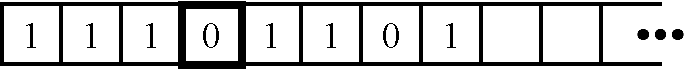
\includegraphics[width=0.5\linewidth]{figures/single-tape-turing-machine.pdf}
    \caption[The tape of a single-tape Turing machine in an arbitrary state.]{The tape of a single-tape Turing machine in an arbitrary state. Note that any multi-tape Turing machines can be efficiently simulated by a single-tape Turing machine~\cite{hartmanis1965computational}, so complexity classes are not affected by changing between single-tape and multi-tape machines.}
    \label{fig:single-tape-turing-machine}
\end{figure}

Everything that can be computed on models of computations we use these days can be computed on a Turing machine~\cite{dershowitz2008natural}.
This hypothesis is known as the Church-Turing thesis.
Related to the Church-Turing thesis is the extended Church-Turing thesis, which states that any physically realizable model of computation can be efficiently simulated on a Turing machine.
That is, can a Turing machine simulate any model of computation in polynomial time?
The quantum computational model brings doubt to this claim.
It is known that quantum computers can efficiently simulate a Turing machine, so they are at least as powerful as classical computers~\cite{bennett1973logical}.
However, there appears to be no efficient algorithm for simulating a quantum computer on a Turing machine~\cite{deutsch1985quantum}.
Furthermore, \textcite{arute2019quantum} experimentally demonstrated a quantum computer sampling from a probability distribution intractable by a classical computer.

\subsection{Complexity Classes}
Complexity classes are sets of computational problems that share some common feature with regard to the computational resources they need to solve some problem~\cite{arora2009computational}.
They are defined in terms of a type of computational problem, computational model, and a bounded resource such as time or space.
In general, most complexity classes describe decision problems solvable by deterministic Turing machines --- though many complexity classes are defined in terms of other types of problems and computational models.
This report mainly focuses on complexity classes involving Turing machines and quantum Turing machines.

The class $\P$ contains all decision problems solvable by a deterministic Turing machine in polynomial time.
Problems that fall under this class are often referred to as tractable or easy problems~\cite{cormen2009introduction}.
The class $\NP$ (non-deterministic polynomial) contains all problems \emph{verifiable} by a deterministic Turing machine in polynomial time.
Equivalently, $\NP$ can be thought of as all problems solvable in polynomial time by a non-deterministic Turing machine.
A non-deterministic Turing machine is a variant of a Turing machine which is not entirely determined by its input and transition function, but can choose from a set of possible transitions when transitioning.
One could then define $\NP$ as consisting of two phases: first, a non-deterministic Turing machine makes a guess about the solution, and then a second, deterministic Turing machine verifies if the guess is correct.
It is clear that $\P \subseteq \NP$, because if you can solve a problem in polynomial time, you can also verify it in polynomial time.
A still unsolved and important question in computer science is whether $\P = \NP$?
That is, can all problems that can be verified in polynomial time also be solved in polynomial time?

In computer science, it is sometimes possible to speed up computation using randomness.
These kinds of algorithms are referred to as probabilistic algorithms and are defined in terms of a probabilistic Turing machine.
A probabilistic Turing machine is a non-deterministic Turing machine that can choose from a set of possible transitions according to some probability distribution when transitioning.
The probabilistic equivalent of $\P$ is $\BPP$ (bounded-error probabilistic polynomial time) and contains all decision problems solvable by a probabilistic Turing machine in polynomial time where a bounded error rate of $1/3$ is allowed.
Since a non-deterministic Turing machine can efficiently simulate a deterministic Turing machine, $\P \subseteq \BPP$.
There are problems to be known in $\BPP$ and not in $\P$, but the number of such problems is decreasing, and \textcite{goldreich2011world, nisan1994hardness} even argue that $\P = \BPP$.

How do quantum computers relate to these complexity classes?
Quantum computers are probabilistic computational devices, and its complexity class equivalent to $\P$ can be defined by replacing the probabilistic Turing machine from $\BPP$ with a quantum computer.\footnote{Note that quantum computers are not simply probabilistic Turing machines as will be shown in the following sections.}
The class $\BQP$ (bounded-error quantum polynomial time) consists all decision problems solvable by a quantum computer in polynomial time where a bounded error rate of $1/3$ is allowed.
It is known that there are $\NP$ problems that can be efficiently solved on a quantum computer like integer factorization, discrete logarithms, and quantum many-body simulation.
As mentioned in the previous section, quantum computers can also solve all problems in $\P$ efficiently, so $\P \subseteq \BQP$.
Furthermore, quantum computers are more powerful than classical probabilistic computers~\cite{bernstein1997quantum}, giving $\BPP \subseteq \BQP$.
How $\BQP$ relates to $\P$ and $\NP$ exactly is still unknown, however, it seems unlikely that $\BQP = \NP$~\cite{aaronson2010bqp}.

\begin{figure}[ht]
    \centering
    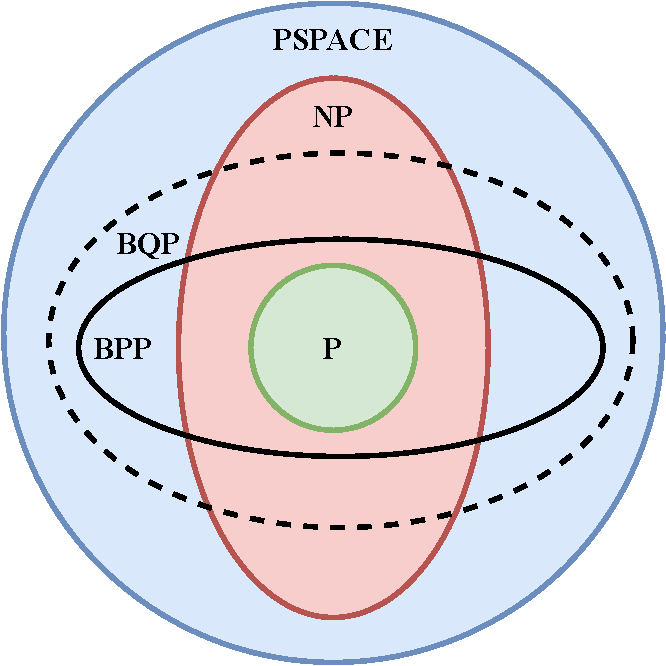
\includegraphics[width=0.5\linewidth]{figures/complexity-classes-hierarchy.pdf}
    \caption[An overview of the hierarchy of the complexity classes discussed.]{An overview of the hierarchy of the complexity classes discussed. This graphic assumes $\P \neq \NP$, $\P \neq \BPP$, and $\P \subseteq \BPP \subseteq \BQP$. $\PSPACE$ is the space equivalent of $\P$, containing all problems that can be solved in polynomial space by a deterministic Turing machine.}
    \label{fig:complexity-classes-hierarchy}
\end{figure}

\section{Quantum Mechanics}
In classic information theory, the smallest unit of information is the bit.
A bit can be in one of two states: 0 or 1.
Quantum information is built upon an analogous concept: the quantum bit, or qubit.
Qubits are physical objects that appear in nature on the scale of atoms and subatomic particles.
A qubit can be any two-state quantum-mechanical system such as the spin of an electron, which can be spin up or down, or the polarization of a photon, which can be horizontally of vertically polarized.
In this report, qubits will be treated as abstract mathematical objects as the physical realization of qubits is beyond the scope of this work.

\subsection{Quantum States}
The state of a qubit is denoted as follows:
\begin{equation} \label{eqn:qubit-state}
\ket{\psi} = \alpha_0\ket{0} + \alpha_1\ket{1}.
\end{equation}
Quantum states are often described using Dirac notation \ket{\,\cdotp\,}, which describes a column vector in $\mathbb{C}^n$.
The states $\{\ket{0}, \ket{1}\}$ are the computational basis states which are defined as $(\begin{matrix}1 & 0\end{matrix})^T$ and $(\begin{matrix}0 & 1\end{matrix})^T$ respectively, and form an orthonormal basis for this vector space.
The values $\alpha, \beta \in \mathbb{C}$ are the state's probability amplitudes, and cannot be examined directly.\footnote{The field of quantum tomography focuses on recovering these values through multiple measurements, but this requires prior knowledge about the system~\cite{d2003quantum}.}
When measuring a qubit, it collapses probabilistically to one of the basis states.
The probability of it collapsing to \ket{0} is given by the absolute square $|\alpha_0|^2$, and the probability of it collapsing to \ket{1} is given by $|\alpha_1|^2$.
As these values are probabilities, they should be normalized: $|\alpha_0|^2 + |\alpha_1|^2 = 1$.
Formally, a qubit can be thought of as a unit vector in a two-dimensional Hilbert space.

A qubit differs from a classical bit in that it can be in a linear combination, or superposition of states.
While a bit can be only be in the state 0 or 1, a qubit can be in one of infinitely many superpositions of states.
However, the laws of quantum mechanics restricts direct access to the probability amplitudes of a state.
Instead, when measuring a qubit, it collapses to basis state \ket{j} with probability $|\alpha_j|^2$.
For example, consider the state
\begin{equation} \label{eqn:plus-state}
\ket{+} = \dfrac{1}{\sqrt{2}}\left(\ket{0} + \ket{1}\right).
\end{equation}
This state has equal probability of measuring \ket{0} and \ket{1}, as $|1/\sqrt{2}|^2 = 1/2$.
Note that measurement changes the state of a qubit: if the state from \Cref{eqn:plus-state} is measured as \ket{1}, the superposition is lost and the state becomes \ket{1}.

A helpful geometric interpretation of a qubit's state can be obtained by rewriting \Cref{eqn:qubit-state} as
\begin{equation}
\ket{\psi} = e^{i\delta} \left(\cos\dfrac{\theta}{2}\ket{0} + e^{i\varphi}\sin\dfrac{\theta}{2}\ket{1}\right),
\end{equation}
where $\delta, \theta, \varphi \in \mathbb{R}$.
The global phase $e^{i\delta}$ can often be ignored, as $\forall \delta \in \mathbb{R} : |e^{i\delta}| = 1$, so it does not impact measurement outcome.
Simplifying then, the state of a qubit can be written as
\begin{equation}
\ket{\psi} = \cos\dfrac{\theta}{2}\ket{0} + e^{i\varphi}\sin\dfrac{\theta}{2}\ket{1}.
\end{equation}
Here, $\theta$ and $\varphi$ define a point on a three-dimensional sphere (\Cref{fig:bloch-sphere}).
\begin{figure}[ht]
    \centering
    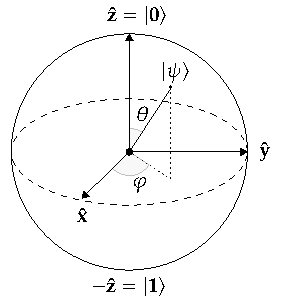
\includegraphics[width=0.35\linewidth]{figures/bloch-sphere.pdf}
    \caption[Bloch sphere representation of a qubit's state.]{Bloch sphere representation of a qubit's state.}
    \label{fig:bloch-sphere}
\end{figure}
While this visualization is limited to a single qubit, it can be a useful visual to build intuition.
For example, the \ket{+} state described in \Cref{eqn:plus-state} can be thought of as being exactly between \ket{0} and \ket{1} on the Bloch sphere.

The amount of probability amplitudes grows exponentially with the amount of qubits.
Consider a two-qubit system which lives in a $2^2=4$-dimensional Hilbert space spanned by the computational basis states $\left\{\ket{00}, \ket{01}, \ket{10}, \ket{11}\right\}$.
This state is defined by the linear combination
\begin{equation} \label{eqn:two-qubit-state}
\ket{\psi} = \alpha_0\ket{00} + \alpha_1\ket{01} + \alpha_2\ket{10} + \alpha_3\ket{11}.
\end{equation}
Again, unlike classical bits who can only be in one state at a time, this qubit can be in a superposition of all four states.
The normalization condition still applies for \Cref{eqn:two-qubit-state}: $\sum_{i=0}|\alpha_i|^2 = 1$.
Single-qubit states can be combined to form multi-qubit states by taking the tensor product of the two states.
Given states $\ket{\psi} = \alpha_0\ket{0} + \alpha_1\ket{1}$ and $\ket{\varphi} = \beta_0\ket{0} + \beta_1\ket{1}$:
\begin{equation} \label{eqn:tensor-product-states}
\begin{aligned}
\ket{\psi} \otimes \ket{\varphi} &= \begin{pmatrix}\alpha_0 \\ \alpha_1\end{pmatrix} \otimes \begin{pmatrix}\beta_0 \\ \beta_1\end{pmatrix} \\
&= \begin{pmatrix}\alpha_0\begin{pmatrix}\beta_0 \\ \beta_1\end{pmatrix} \\ \alpha_1\begin{pmatrix}\beta_0 \\ \beta_1\end{pmatrix}\end{pmatrix} \\
&= \begin{pmatrix}\alpha_0\beta_0 \\ \alpha_0\beta_1 \\ \alpha_1\beta_0 \\ \alpha_1\beta_1\end{pmatrix} \\
&= \alpha_0\beta_0\ket{00} + \alpha_0\beta_1\ket{01} + \alpha_1\beta_0\ket{10} + \alpha_1\beta_1\ket{11}.
\end{aligned}
\end{equation}
The relative phases of $\alpha_0, \alpha_1$ and $\beta_0, \beta_1$ are responsible for the quantum mechanical property of interference.
When the phase of $\alpha_j$ and $\beta_j$ is the same, they will interfere constructively and increase the probability amplitude for that state.
On the other hand, if $\alpha_j$ and $\beta_j$ have opposite phases, they will interfere destructively and decrease the probability amplitude for that state.

Not all multi-qubit systems can be expressed as a tensor product of individual states as shown in \Cref{eqn:tensor-product-states}.
Consider the following state:
\begin{equation} \label{eqn:bell-state}
\ket{\Phi^+} = \dfrac{1}{\sqrt{2}}\left(\ket{00} + \ket{11}\right).
\end{equation}
This state cannot be expressed as a tensor product of two individual states, because that would imply $\big(\alpha_0\beta_0 = \alpha_1\beta_1 = 1/\sqrt2\,\big) \wedge \big(\alpha_0\beta_1 = \alpha_1\beta_0 = 0\big)$, which is a contradiction.
States like $\ket{\Phi^+}$ are referred to as entangled states.
Entanglement is the quantum phenomena of correlation in measurement outcomes.
For example, when measuring the state $\ket{\Phi^+}$ from \Cref{eqn:bell-state}, the only two possible measurement outcomes are \ket{00} and \ket{11}.
So by measuring one qubit, one also knows the state of the other qubit.

\subsection{State Evolution}
The evolution of a closed quantum system is described by a unitary transformation~\cite{nielsen2002quantum}.\footnote{In this report, a perfectly closed system is assumed, even though in reality all systems interact somewhat with other systems.}
A state \ket{\psi} at time $t_1$ is related to state \ket{\psi'} at time $t_2$ by a unitary operator $U$:
\begin{equation}
\ket{\psi'} = U\ket{\psi}.
\end{equation}
The unitary nature of these operators implies $UU^\dagger = U^\dagger U = I$, where $^\dagger$ is the conjugate transpose and $I$ the identity matrix.
Single-qubit operators can be represented as $2 \times 2$ complex-valued unitary matrices.
A common single-qubit operator is the Pauli-$X$ operator which transforms a state $\alpha_0\ket{0} + \alpha_1\ket{1}$ to $\alpha_1\ket{0} + \alpha_0\ket{1}$.
It is part the set of Pauli matrices:
\begin{equation}
X = \begin{pmatrix}
0 & 1 \\
1 & 0
\end{pmatrix}, \hspace*{5mm}
Y = \begin{pmatrix}
0 & -i \\
i & \phantom{-}0
\end{pmatrix}, \hspace*{5mm}
Z = \begin{pmatrix}
1 & \phantom{-}0 \\
0 & -1
\end{pmatrix}.
\end{equation}
These matrices are ubiquitous in the study of quantum computation and information.
Another useful and common operator is the Hadamard operator:
\begin{equation}
H = \dfrac{1}{\sqrt2}
\begin{pmatrix}
1 & \phantom{-}1 \\
1 & -1
\end{pmatrix},
\end{equation}
which maps the computational basis states to an equal superposition state.

The Pauli-$Z$ operator is part of the $Z$-rotation operators family.
The general form for $Z$-axis rotation can be described as follows:
\begin{equation}
R_z(\theta) = \begin{pmatrix}
1 & 0 \\
0 & e^{i\theta}
\end{pmatrix}.
\end{equation}
From this definition follows that $Z = R_z(\pi)$.
Other common $Z$-axis rotation operators are $S = R_z(\pi/2)$ and $T = R_z(\pi/4)$.
Note that all $Z$-axis rotation operators only influence the \ket{1} amplitude of the state:
\begin{equation}
\begin{aligned}
R_z(\theta)\ket{0} &= \ket{0} \\
R_z(\theta)\ket{1} &= e^{i\theta}\ket{1}.
\end{aligned}
\end{equation}

Multi-qubit operators act on two or more qubits.
They are required for creating entangled states.
Two common two-qubit operators are the $CNOT$ and $CZ$ operators.
The $CNOT$ operator can be thought of as a controlled-$X$ operator, which applies an $X$ operation on the target qubit if the control qubit is in the \ket{1} state.
Equivalently, the $CZ$ operator applies a $Z$ operation on the target qubit if the control qubit is \ket{1}.
Their matrix representations are as follows:
\begin{equation}
CNOT = \begin{pmatrix}
1 & 0 & 0 & 0 \\
0 & 1 & 0 & 0 \\
0 & 0 & 0 & 1 \\
0 & 0 & 1 & 0 \\
\end{pmatrix}, \hspace*{5mm}
CZ = \begin{pmatrix}
1 & 0 & 0 & \phantom{-}0 \\
0 & 1 & 0 & \phantom{-}0 \\
0 & 0 & 1 & \phantom{-}0 \\
0 & 0 & 0 & -1 \\
\end{pmatrix}
\end{equation}

\subsection{Measurement}

\section{Quantum Computation}